\documentclass{article}

\setlength{\parindent}{0pt}
\usepackage[round]{natbib}
\usepackage{listings}
\usepackage{array}

\usepackage{graphicx}
\graphicspath{ {./images/} }

\title{Simulation of Tree Growth}
\date{2020-12-01}
\author{Eric Ekström}
	
\begin{document}
	
	\pagenumbering{gobble}
	\maketitle
	\newpage
  	
  	\section*{Abstract}
  	
  	\newpage
  	\tableofcontents
  	\newpage
  	\pagenumbering{arabic}

  	\section{Introduction}
  		 
  	\section{Background}
  		
  		TODO!
  		
  		\subsection{Tree Structure and Terminology}
  			This section covers the terminology used when describing trees. The choice of language is based on the description of trees by \citep{barthelemy2007plant}. \\
  			
  			A tree consists of a number of nodes. Each node supports nodes further out in the tree.
  			
  			\begin{itemize}
  				\item A \textit{node} is the main component of the tree. It supports at least a bud, another node or a leaf. A node combined with an internode is called a \textit{metamer}. \citep{barthelemy2007plant}
  				\item An \textit{internode} is the section of stem between two nodes.
  				\item The \textit{lateral branch} is a supported node that is connected at an angle  to the supporting node.
  				\item The \textit{main branch} is a supported node that has the same angle as the supporting node.
  				\item \textit{Buds} are potential points for expansion of new nodes. A lateral bud is located at the node that already has a main branch. An apical bud is located at a node that has no branches to support.
  				
  			\end{itemize}
  			
  			For this project, a tree grows by shooting a number of new metamers from a bud. This is called rhythmic growth and is the more commonly observed method of growth in nature. \citep{barthelemy2007plant} The fate of a bud and the number of new metamers depends on a number of factors. For this project, only a simulated light resource was considered.\\
  			
  			A node is given an order based on the number of node below it. A node without a supporting node has order 1.
  		\subsection{Volumetric Light Scattering}
  			Volumetric light scattering (also called "godrays" or "crepuscular rays") is a light phenomenon that occurs when the mixture of gas and molecules in the air is just right. This causes light to be rayleigh-scattered and creates visual sun beams through the air. (See Figure \ref{fig:godrayexample}.)
  			
  			\begin{figure}[h!]
  				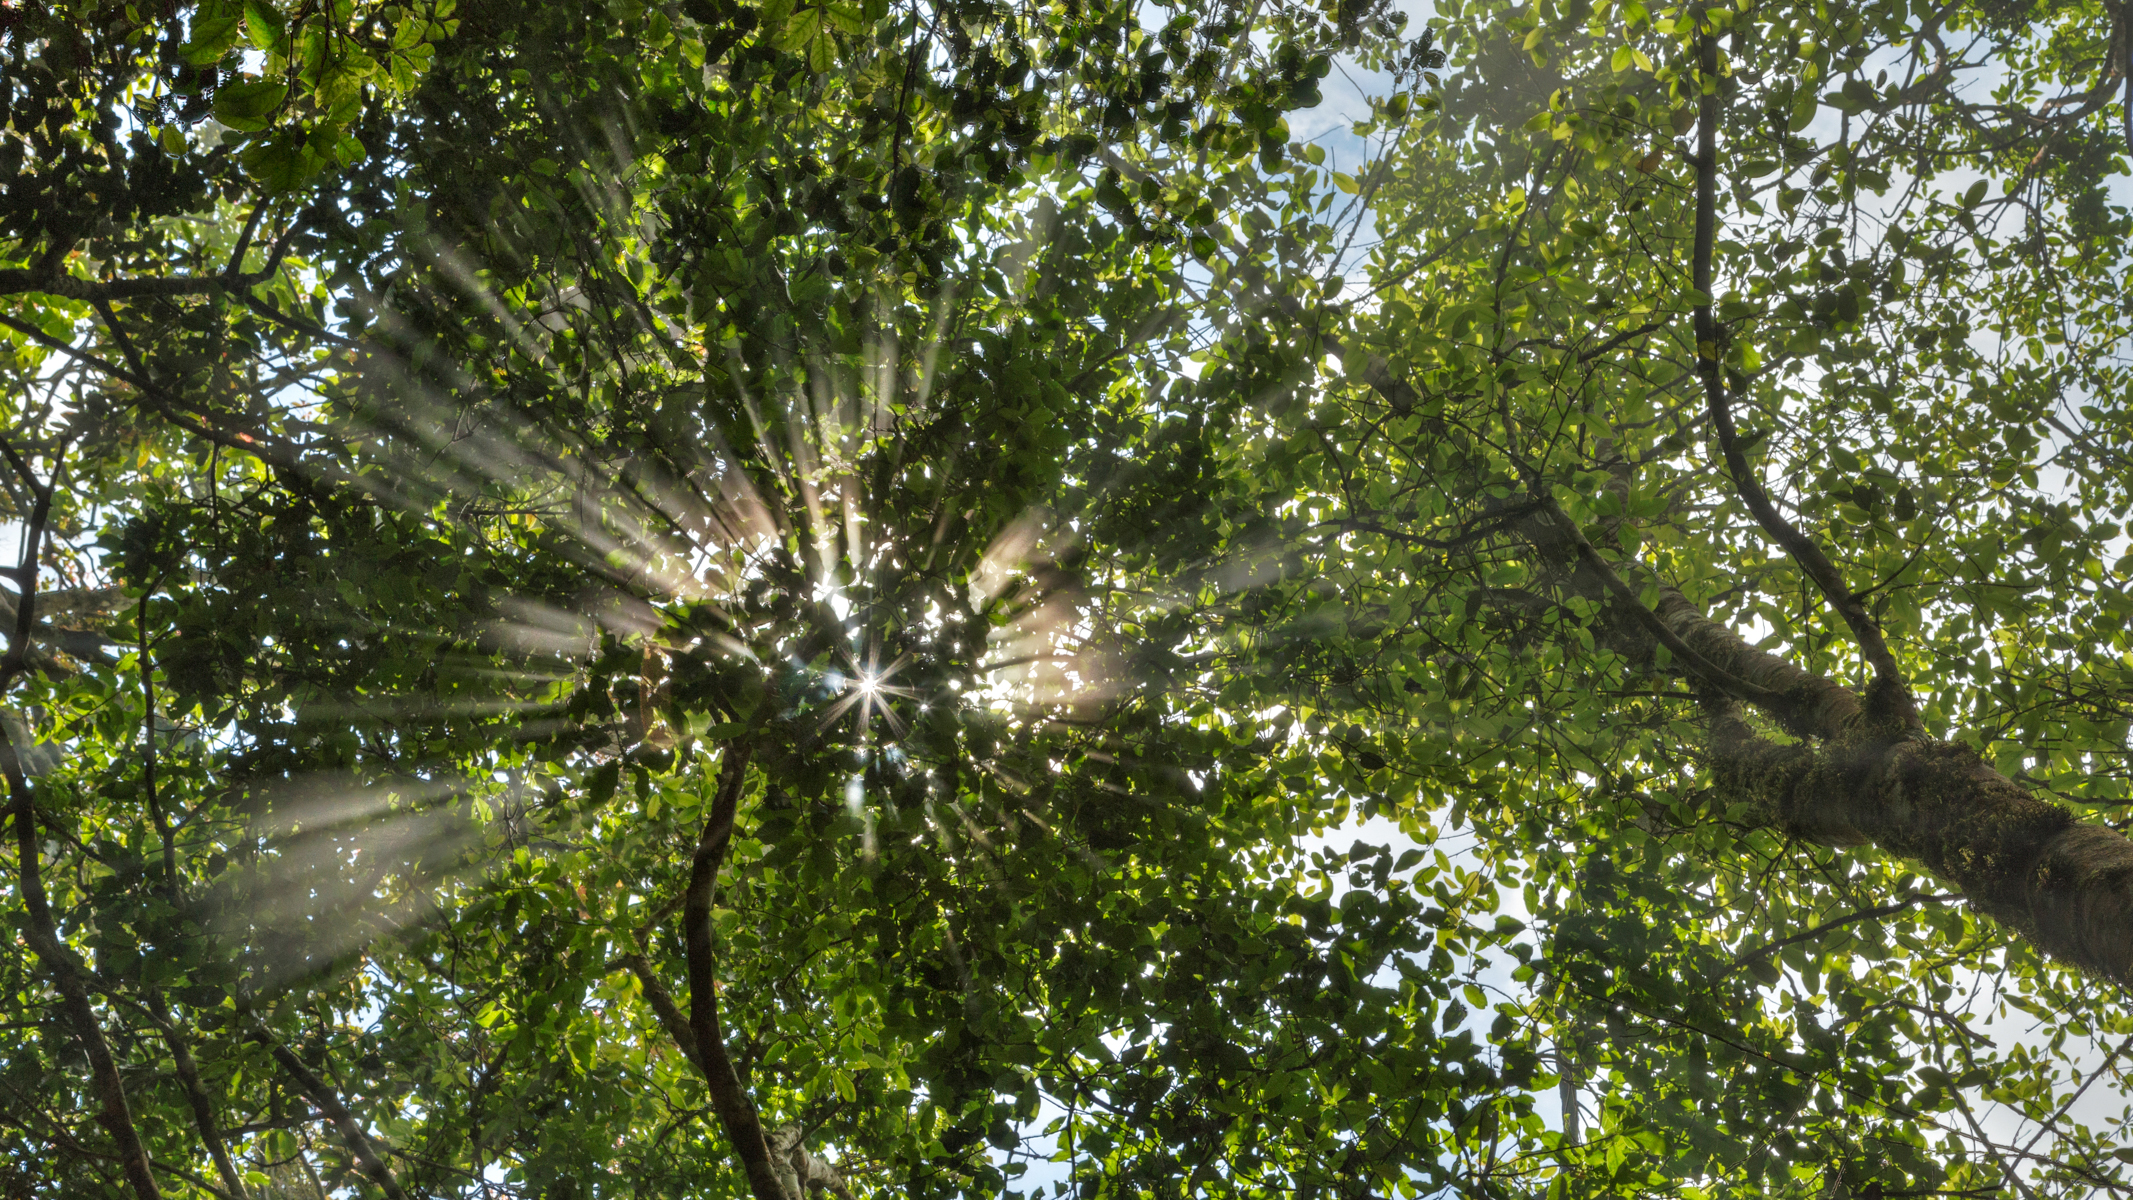
\includegraphics[scale=0.7]{godrays}
  				\caption{An example of volumetric light scattering. (Sunshine Kodai Kanal, Manoj K Racherla, 2013)}
  				\label{fig:godrayexample}
  			\end{figure}
  			
  		
  			
  	\section{Method}
  		\subsection{Tree Generation}
  			
  			TODO: vad är ett träd dååå
  			
  			\subsubsection*{Algorthim outline}
  			
  			The tree generation algorithm used the same basic steps as described by Wojciech Palubicki. \citep{palubicki2009self}
  			
  			\begin{enumerate}
  				\item Calculate the amount of light resources available in the tree.
  				\item Redistribute light resource and create new nodes.
  				\item Update the branch radii for each node.
  				\item Calculate which nodes are a liability, and shed these.
  			\end{enumerate}
  		
  			\subsubsection*{Calculation of light resources}
  			
  				Light resources are collected from each node and saved in the base of the tree. Each node contribute with resources if it has either a lateral or apical bud. The size of the contribution is calculated according to Equation \ref{eq:lightres} as proposed by \cite{yi2018tree}. \textit{T} and \textit{$T_0$} is the current time and the creation time of the node respectively, \textit{l} is the light that hits the current node based on conditions around it and $\sigma$ is a controllable parameter.
  				
  				\begin{equation}
  					\label{eq:lightres}
  					Q = l^{{(T-T_0)}^\sigma}
  				\end{equation}
  				
  				Each node also has a cost associated with it. This is the amount of resources it takes to keep the node alive as discribed by \cite{mvech1996visual}. The equation for calculating this factor is shown in Equation \ref{eq:nodecost}. \textit{BM} and BE are control parameters. This factor is subtracted from the light resources in each node before the result is propagated to the supporting node. 
  				
  				\begin{equation}
  					\label{eq:nodecost}
  					BM * {\frac{radius}{default\_radius}}^{BE}
  				\end{equation}
  				
  			\subsubsection*{Shadow propogation for node light calculation}
  				
  				The variable \textit{l} in equation \ref{eq:lightres} is the amount if light that reach a node and is calculated by considering the nodes already around it. This is done by dividing the space into \textit{voxels} of fixed size. Each voxel saves a float value describing how shadowed the point is. When a new node is added to the tree, it also updated the voxels around it. Specifically, a pyramid of voxels (with the voxel containing the new node at the top) are updated according to Equation \ref{eq:shadowprop}. \textit{a} and \textit{b} are controllable parameters and \textit{q} is the number of voxels down from the top of the pyramid. \citep{palubicki2009self}
  				
  				\begin{equation}
  					\label{eq:shadowprop}
  					s = s_{prev} + a*b^{-q}
  				\end{equation}
  			
  			\subsubsection*{Redistribution of light resources}
  				An adapted version of the Borchert-Honda (BH) model \citep{borchert1984control} was used to redistribute resources to each node. The BH model was originally developed to control distribution of growth-inducing resources. \cite{palubicki2009self} adapted the BH model by using the collected light resources to guide the redistribution of resources. Equation \ref{eq:vm} and \ref{eq:vl} show how the light resources are distributed between the main branch and the lateral branch  based on the amount of resources collected by each node. $Q_m$ and $Q_l$ is the amount of light resources collected by each of the branches and $\lambda$ is a parameter that can be set by the user.
  			
	  			\begin{equation}
	  				\label{eq:vm}
	  				v_m = v\frac{\lambda Q_m}{\lambda Q_m + (1 - \lambda)Q_l}
	  			\end{equation}
	  			
	  			\begin{equation}
	  				\label{eq:vl}
	  				v_l = v\frac{(1 - \lambda) Q_l}{\lambda Q_m + (1 - \lambda)Q_l}
	  			\end{equation}
	  			
	  			The number of new metamers created from a bud is the integer part of the amount of resources that reach the bud. Three factors are considered when deciding the direction of the new branch; direction of the parent node, the optimal growth direction, and a tropism factor. The tropism factor, $\tau$, simulate how much the branches bend down due to gravity. The optimal growth direction  is found as the neighboring shadow voxel with the lowest value. These three factors are combined to the final growth direction according to Equation \ref{eq:growthdir}. \citep{palubicki2009self}
	  			
	  			\begin{equation}
	  				\label{eq:growthdir}
	  				growth\_dir = 0.8 * parent\_dir + 0.2 * optimal\_dir + \tau
	  			\end{equation}
	  			
	  		\subsubsection*{Update branch radii}
	  			
	  			The radius of each branch is updated to support the weight of the branches above it according to Equation \ref{eq:radius}, where $r_m$ and $r_l$ are the new radius of the supported branches. If no supported branch is present, the default branch radius is used. \citep{mvech1996visual}
	  			
	  			\begin{equation}
	  				\label{eq:radius}
	  				r = \sqrt{r_m^2 + r_l^2}
	  			\end{equation}
	  			
	  		\subsubsection*{Calculate shedding branches}
	  			
	  			A branch is shedded if the light resource flowing through it is negative and the number of supported buds are less than a threshold.
	  			\citep{mvech1996visual}
  			
  		\subsection{Volumetric Light Scattering}
  		
  			Volumetric light scattering was done as a post-process shader using the method described by Kenny Mitchell \citep{mitchell}. \\
  			
  			The post-process shader combines the normal render pass with a render pass where the sun is rendered as a single color, and all other objects are then rendered black. This gives an image with color only where the sun is visible from the cameras perspective. \\
  			
  			The post-process shader sums samples of the volumetric light scattering pass from the current fragment point to the position of the sun. The samples are exponentially weighted where the samples close to the sun are weighted higher. The equation used for weighting samples is shows in Equation \ref{eq:godray}. 
  			
  			\begin{equation}
  				\label{eq:godray}
  				L = exposure * \sum_{i = 0}^{n} decay^i * weight * \frac{sample}{n}
  			\end{equation}
  			
  			\textit{n} is the number of samples between the fragment position and the sun position, \textit{decay} is the exponentially decaying factor that dissipated the contribution from each sample. The \textit{exposure} and \textit{weight} factors are simply scale factors that increase or decrease the final light. \\
  			
  			The final factor \textit{L} for each pixel is then added to the final color of the normal pass for that pixel. The shader code used for volumetric light scattering can be found in appendix \ref{appendix:godray}.
  		
  		\subsection{Shadow Mapping}
  			Shadow mapping is a popular technique for generating good shadows in a scene. It works in two steps; first render the scene from the perspective of the light source, then render the scene as normal using the first render to calculate which fragments are in shadow. \citep{ragnemalm2015so} \\
  			
  			The purpose of the first render pass is to generate a map of depth values for each point that the camera can see. These depth values are then used in the second pass to calculate shadows. If the distance to the camera from the current fragment is greater then the depth value saved in the depth map, there is another fragment somewhere in between the fragment and the sun and the fragment is therefor in shadow. \citep{ragnemalm2015so}
  			
  			\subsubsection*{Implementation}
  				
  				A framebuffer with only a depth attachment was used to generate the depth map. Since the only part of interest is the depth values, the used fragment shader can be empty and just write the depth values to the z-buffer. The vertex shader is the same as would be used in a normal scene. \\
  				
  				The implementation for this project only create shadows from directional light sources. Because of this, a orthographic projection matrix was used. This gives a more realistic result by pretending that all light hits the scene as parallel lines. The position of the light source still have to de specified since it is needed to calculate the distance from a fragment. \\
  				
  				This method will generate a number of different artifacts that have to be addressed. The first and most obvious is "shadow acne". This is caused by the fact that the resolution of the shadow map is limited and there is more than one fragment on a surface that sample from the same point in the shadow map. Even though all the fragment on a surface should be lit, only the fragments that happen to have its distance saved in the shadow map are actually lit. This can be solved by adding a small offset when comparing the distance with the depth map. \\
  				
  				The next problem that has to be handled is the fragments that are outside the depth map. here we simply set the texture as "clamp to edge" and set the border of the depth texture to 1. The same problem arise when a fragment is beyond the outer limit of the projection matrix. The solution is to set the shadow to 0 if the distance is greater than the furthest allowed distance.
  				
  				For a full implementation of the shader code used for shadow mapping, see appendix \ref{appendix:shadow}.
  				
  	\section{Result}
  		
  		
  		
  		
  		\subsubsection*{Tree Parameters}
  		
  		Table \ref{table:param} shows the parameters that were used and how they affect the look of the tree.
  		
  		\begin{table} [!h]
  			\begin{center}
  				\begin{tabular}{ | c | m{5cm} | c | } 
  					\hline
  					Name & Effect & Reasonable range \\
  					\hline
  					\hline
  					lambda, $\lambda$ & Branch bias. Larger value gives priority to main branches. & 0.4 - 0.5 \\ 
  					\hline
  					sigma, $\sigma$ & Light conversion rate. Larger values increase the amount of light an older node can pick up. & 0 - 1\\ 
  					\hline
  					tropism, $\tau$ & Larger value bend branches more towards the ground. & 0.01 - 0-5 \\ 
  					\hline
  					BM & Branch maintenance coefficient & 0.01 - 0.5 \\ 
  					\hline
  					BE & Branch maintenance exponent &  $>$1\\ 
  					\hline
  					$N_{min}$ & Threshold for branch shedding. & 20 - 50 \\ 
  					\hline
  				\end{tabular}
  				\caption{Table of used tree parameters.}
  				\label{table:param}
  			\end{center}
  		\end{table}
  		
  	\section{Discussion}
  		
  		
  		
  		
  		
  		
  		
  		
  		shadow map - resolution
  		
  	\subsection{Improvements}

	\newpage
	\bibliographystyle{plainnat}
	\bibliography{ref}{}
	
	\newpage
	\appendix
	\section{Shader code for volumetric light scattering}
	\label{appendix:godray}
		
	\begin{lstlisting}[basicstyle=\ttfamily\footnotesize, tabsize=4]
	vec2 delta_tex_coord = vec2(out_tex_coords - sun_pos);
	delta_tex_coord *= 1.0 / float(NUM_SAMPLES) * density;
	
	vec2 tex_coord = out_tex_coords;
	
	float illumination_decay = 1.0;
	vec4 godray_color = vec4(0,0,0,0);
	
	for(int i = 0; i < NUM_SAMPLES; i++)
	{
		tex_coord -= delta_tex_coord;
		
		vec4 s = texture(god_ray_pass, tex_coord);
		
		s *= illumination_decay * weight;
		
		godray_color += s;
		
		// Update exponential decay factor.
		illumination_decay *= decay;
	}
	
	return godray_color * exposure;
	\end{lstlisting}
		
	\section{Shader code for shadow map calculation}
	\label{appendix:shadow}
		
	\begin{lstlisting}[basicstyle=\ttfamily\footnotesize, tabsize=4]
	vec3 proj_coords = frag_pos_light_space.xyz / frag_pos_light_space.w;
	proj_coords = proj_coords * 0.5 + 0.5;

	float current_depth = proj_coords.z;
	
	float bias = max(0.005 * (1.0 - dot(normal, light_dir)), 0.00005);
	float shadow = 0.0;
	vec2 texel_size = 1.0 / textureSize(shadow_map, 0);
	for(int x = -1; x <= 1; ++x)
	{
		for(int y = -1; y <= 1; ++y)
		{
			float depth = texture(shadow_map, proj_coords.xy + vec2(x, y) * texel_size).r; 
			shadow += current_depth - bias > depth ? 1.0 : 0.0;        
		}
	}
	shadow /= 9.0;
	
	if(proj_coords.z > 1.0)
		shadow = 0.0;
	
	return shadow;
		
	\end{lstlisting}
  	
\end{document}
